\section{BPMN-models}
	The following BPMN-models\cite{bpmn} describe how we view the current processes of registering to a course, and complaining on a grade, followed by our suggested changes.
All models are from a student's perspective, as that is what we found most interesting.

\subsection{registering to a course}
		
\begin{figure}[H]
    \centering
    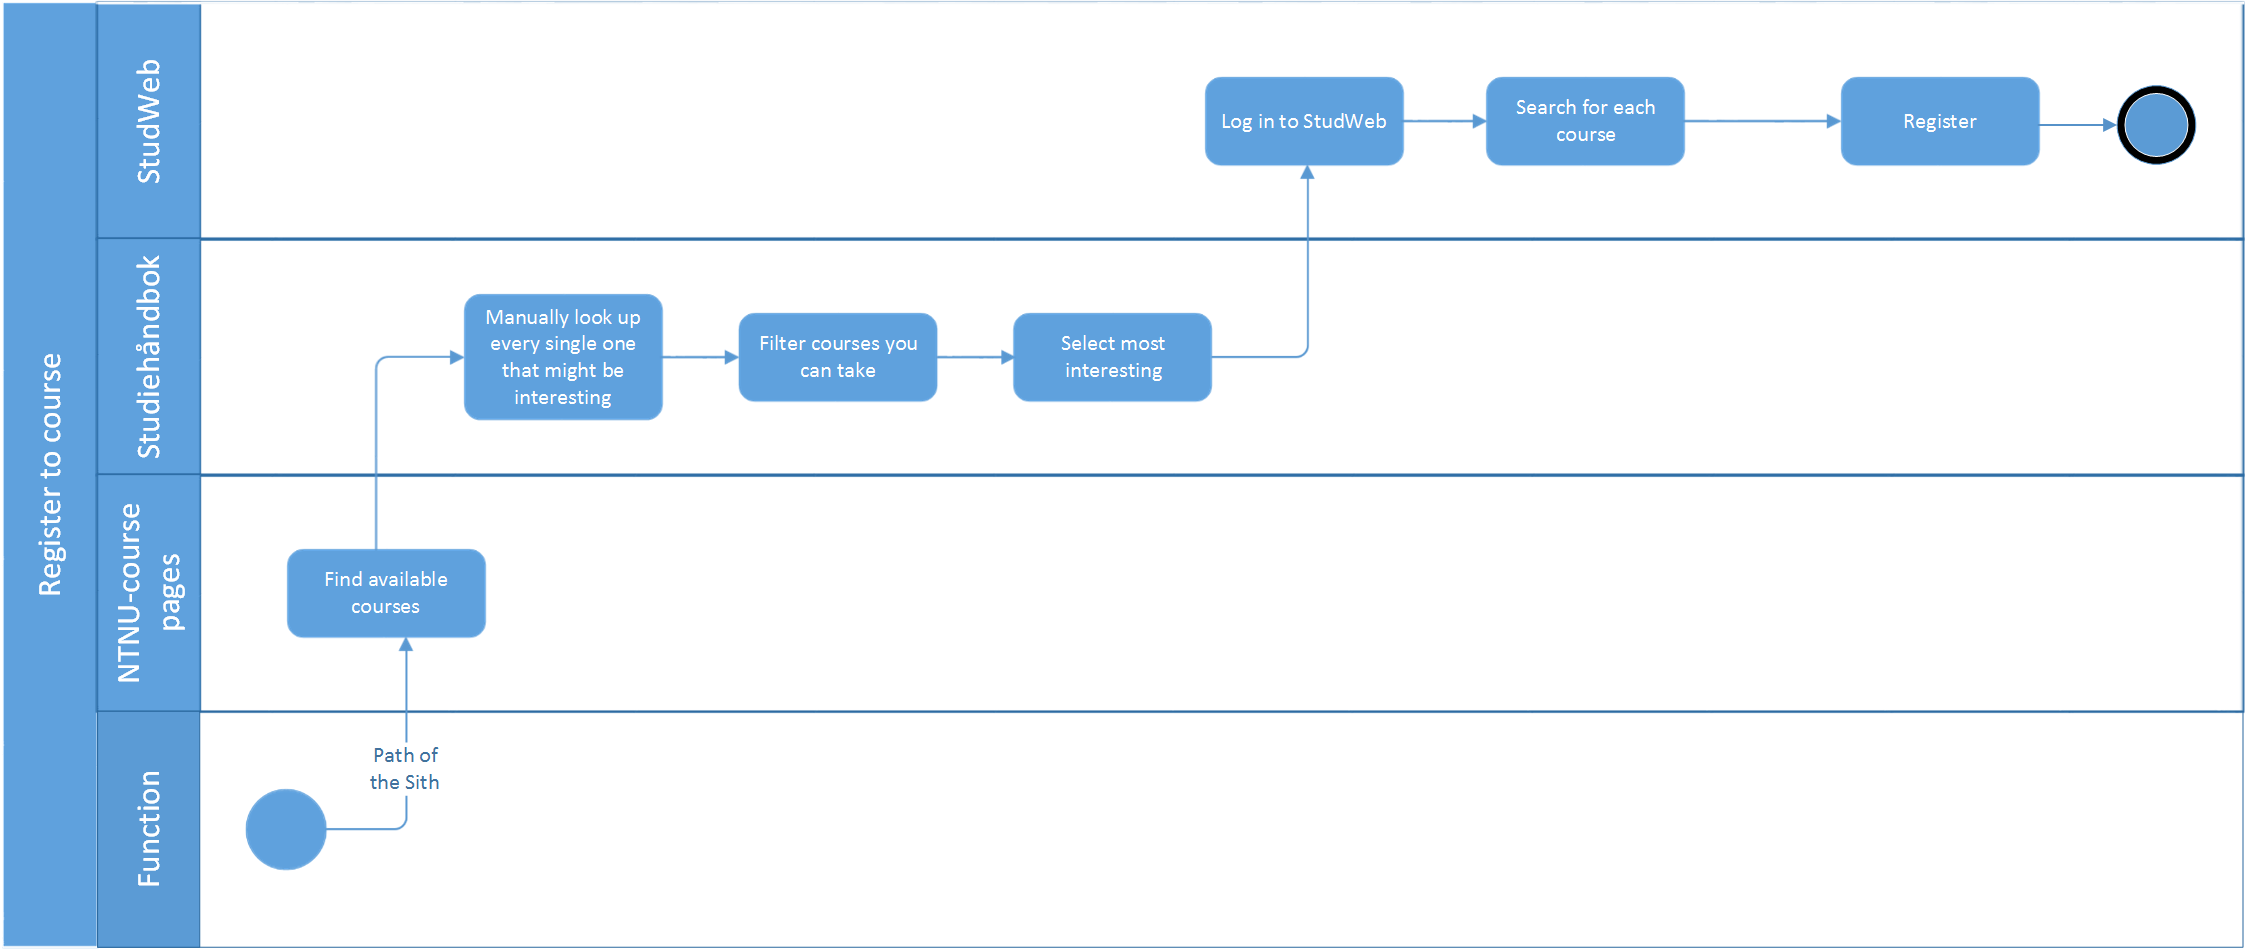
\includegraphics[width=\textheight, angle=-90]{BPMN-register-old}%apparently sets width first and then rotates
    \caption{Our interpretation of the current process of registering to a course.}
    \label{fig:Register-old}
\end{figure}

\begin{figure}[H]
    \centering
    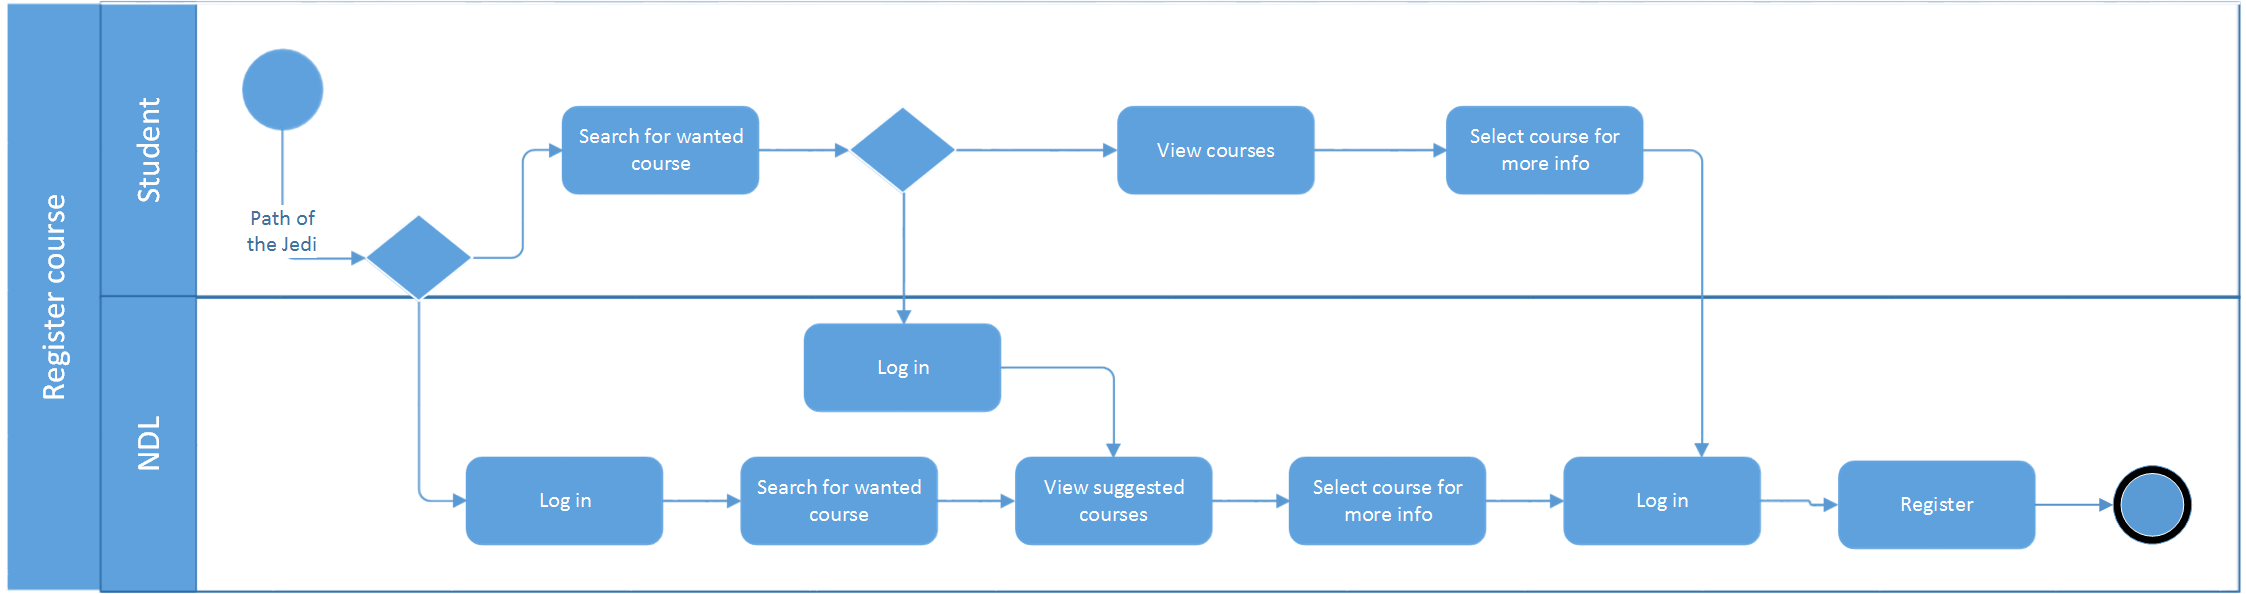
\includegraphics[width=\textheight, angle=-90]{BPMN-register}
    \caption{How we envision our new process of registering to a course to be.}
    \label{fig:Register-new}
\end{figure}

\begin{figure}[H]
    \centering
    \includegraphics[width=\textheight, angle=-90]{BPMN-complain-old}
    \caption{Our interpretation of the current process of complaining on a grade}
    \label{fig:Complain-old}
\end{figure}

\begin{figure}[H]
    \centering
    \includegraphics[width=\textheight, angle=-90]{BPMN-complain}
    \caption{How we envision our new process of complaining to be.}
    \label{fig:Complain-new}
\end{figure}
